\documentclass[12pt]{article}

\usepackage[utf8]{inputenc}
\usepackage[T1]{fontenc}  
\usepackage[francais]{babel}   
\usepackage{fancyhdr}
\usepackage[top=2.5cm,bottom=3.5cm,left=2.5cm,right=2.5cm]{geometry}
\usepackage{lmodern}
\usepackage{listings}
\usepackage{color}
\usepackage{blindtext}
\usepackage[colorlinks=true,urlcolor=black,linkcolor=black]{hyperref}
\definecolor{grey}{rgb}{0.3,0.3,0.3}
\usepackage{graphicx}

\lstset{
language=java,
basicstyle=\footnotesize\ttfamily,
numberstyle=\normalsize,
numbersep=7pt,
keywordstyle=\color{blue},
commentstyle=\color{grey}
}

\newcommand\Titre{TP DASI : If'Routard}
\newcommand\Dater{Pour le 3 avril 2015}
\newcommand{\Numbi}{B3425}
\newcommand{\Membres}{\textsc{Bai} Émilien,
\newline \textsc{Haidara} Mohamed}

\title{\Titre \newline \large Compte Rendu}
\author{Bin\^ome \Numbi{}: \Membres}
\date{\Dater}

\begin{document}

\pagestyle{fancy}
\renewcommand{\footrulewidth}{1pt}
\renewcommand{\headheight}{2cm}
\renewcommand{\contentsname}{Table des matières}



\lhead{\Membres}
\chead{\Titre}
\rhead{\Numbi}

\begin{center}
\begin{LARGE}
\begin{bfseries}

\vspace{1\baselineskip}

\Titre
~\newline~\newline \begin{large} Compte Rendu\end{large}
\end{bfseries}
\end{LARGE}
\end{center}

\tableofcontents

\section*{Introduction}
Lors de ce Tp, nous avons travaillé autours de la création d'une application pour agence de voyage. Cette application est divisée en deux interfaces principales qui sont une IHM client fenêtrée utilisée par les créateurs de voyage pour gérer leur agence et une IHM web permettant aux aux clients de consulter le catalogue des voyages proposés afin d'établir un devis. L'objectif de la première période de TP est de spécifier les IHM et réaliser l'architecture des données et des services nécessaires au fonctionnement de l'application dans les cas d'usages décris par le sujet.

\section{Modèle de domaine}
À la suite de l'analyse des besoins exprimés par le sujet, nous avons établis le modèle de domaine suivant :
\begin{center}
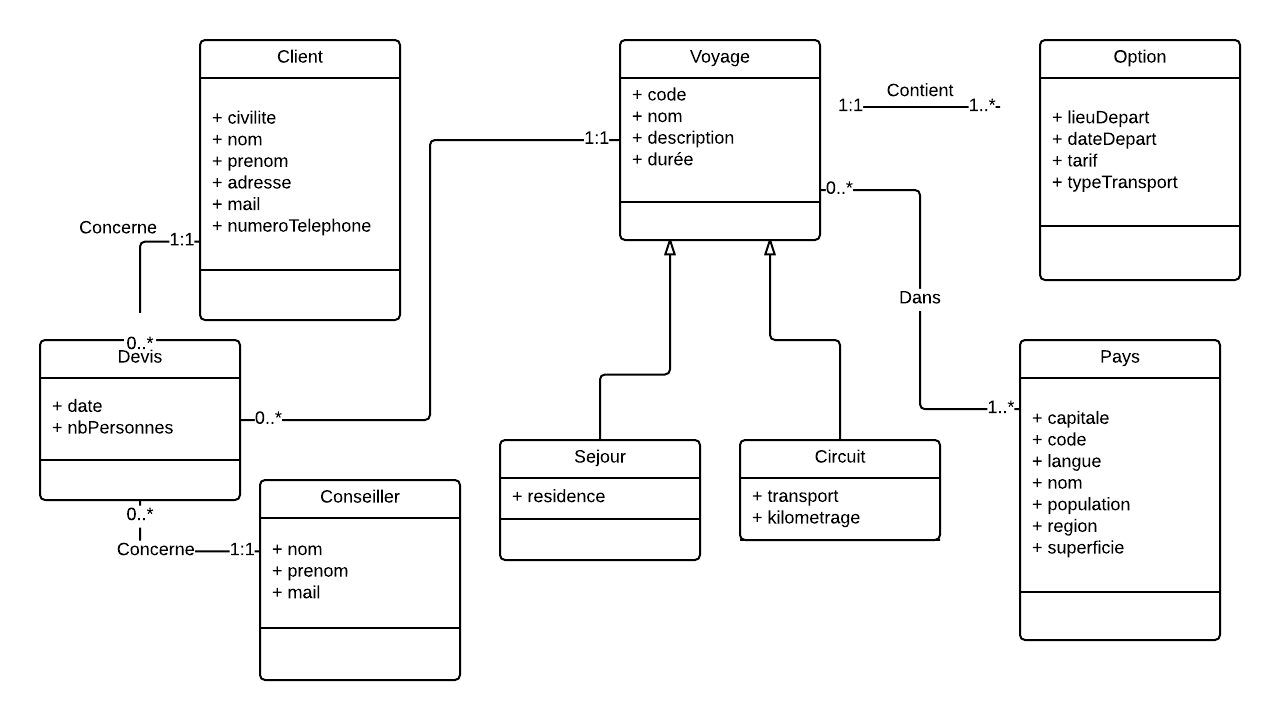
\includegraphics[scale = 0.8]{ModeleDomaine.png}
\newline
Modèle de domaine
\label{fig:ModeleDomaine}
\end{center}
Ce modèle nous permet de stocker toutes les informations nécessaires au fonctionnement de l'application.

\section{Spécification des IHM}
\subsection{IHM Client fenêtrée}
\subsubsection{Présentation}
Cette IHM est celle qui est destinée aux employés de l'agence de voyage. C'est à partir de là qu'il peuvent gérer le catalogue de voyage et éventuellement les devis et informations renseignées sur les pays. Pour ce TP, nous nous sommes limités à  la gestions des voyages. 
\paragraph{Créateur - Connexion}
La première fenêtre à l'ouverture de l'application est une fenêtre de connexion ou l'employé peut s'identifier grâce à son adresse e-mail. Dans le futur, cette identification pourrait permettre de limiter les accès aux fonctionnalités de l'application suivant les catégories d'employés. Elle se présente sous la forme suivante:
\begin{center}
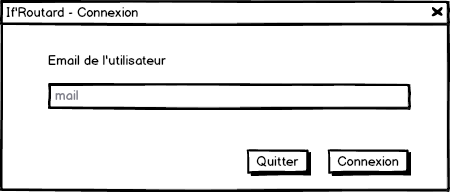
\includegraphics[scale = 0.6]{../Conception_graphique/png_Pour_CR/Createur-00-Connexion.png}
\newline
Créateur - Connexion
\label{fig:Cr-Connexion}
\end{center}
\paragraph{Créateur - Accueil}
Après leur connexion, les employés de l'agence de voyage arrivent sur l'écran d'accueil. À	partir de cette écran, ils peuvent accéder aux différents objets pouvant les intéresser, c'est à dire, les voyages, les devis ou encore les pays (pour une mise à jour des données ou une consultation par exemple). C'est aussi à partir de cette fenêtre qu'ils peuvent se déconnecter de leur compte. Elle se présent sous la forme suivante:
\begin{center}
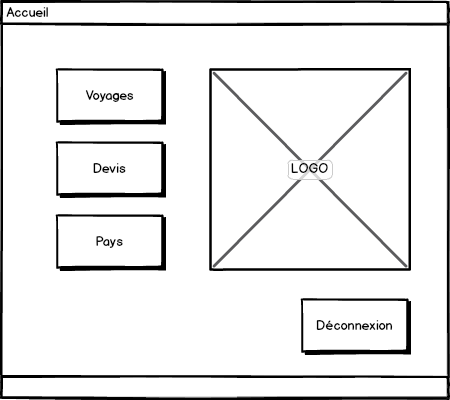
\includegraphics[scale = 0.6]{../Conception_graphique/png_Pour_CR/Createur-10-Accueil.png}
\newline
Créateur - Accueil
\label{fig:Cr-Accueil}
\end{center}

\paragraph{Créateur - Liste Voyage}
À partir de cette fenêtre, les créateurs peuvent rechercher un voyage sur lequel ils souhaitent travailler. Il sélectionnent le voyage qui les intéresse dans la liste 

\subsubsection{ICARs - Client fenêtré}

\subsection{IHM - Client Web}
\subsubsection{Présentation}
\subsubsection{ICARs}

\section{Services}


\end{document}